\documentclass[11pt]{article}

\usepackage{amsmath}
\usepackage{amsfonts}
\usepackage{url}
\usepackage{graphicx}
\usepackage[a4paper,top=1.2in, bottom=1.2in, left=1.2in, right=1.2in]{geometry}
\usepackage{ifthen}

% no indent
\setlength\parindent{0pt}

% points
\newcommand{\points}[1]{
    \ifthenelse{\equal{#1}{1}}
        {\\ \emph{(#1 Point)}}
    % else
        {\\ \emph{(#1 Points)}}
}

\begin{document}

\begin{center}

	\textbf{Exercise 02 for MA-INF 2201 Computer Vision WS17/18	\\
		      23.10.2017					\\
	Submission on 29.10.2017					}

\end{center}

\vspace{0cm}

\begin{enumerate}

	\item	Read the image \texttt{traffic.jpg}, build a Gaussian and Laplacian pyramid and display each layer. 
		For the Gaussian pyramid compare two versions:
		\begin{itemize}
			\item         using \texttt{cv::pyrDown} and \texttt{cv::buildPyramid}
			\item without using \texttt{cv::pyrDown} and \texttt{cv::buildPyramid}
		\end{itemize}	
		Compute the maximal pixel-wise difference between both versions for each layer.\quad%\\
		\emph{Hint:} the third parameter of \texttt{cv::pyrUp} should be used to guarantee a certain image size.\\
		\emph{(3 Points)}
		
	\item	Blend the image \texttt{apple.jpg} and \texttt{orange.jpg} using Laplacian blending\footnote{For further details you can refer to: \emph{P.Burt and E. Adelson. A Multiresolution Spline With Application to. Image Mosaics. ACM Trans. Graph. 1983}} to obtain an image similar to Fig. \ref{fig:blendedIMG}.\\
		\emph{(5 Points)}
	
					\begin{figure}[hb]
					\vspace*{-2mm}
					\centering
						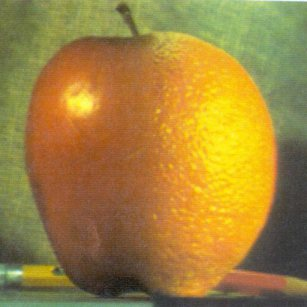
\includegraphics[height=0.28 \linewidth]{blended.png}
					\vspace*{-2mm}
					\caption{Blended image.}\label{fig:blendedIMG}
					\end{figure}

	\item	\begin{sloppypar}
		Read the image \texttt{traffic.jpg} and convert it into a gray image and display it.  
		\begin{itemize}
			\item Compute the gradients using \texttt{cv::sobel}.
			\item Compute the gradient magnitude and gradient direction without using \texttt{cv:cartToPolar} and display both of them.
		\end{itemize}
		\emph{Hint: Use the right value \texttt{ddepth} for \texttt{cv::sobel} to avoid overflow.}
		\\ \emph{(3 Points)}
		\end{sloppypar}
	
	\item	Read the image \texttt{traffic.jpg}, convert it into a gray image, and extract edges using \texttt{cv::Canny}. Display the gray image and the edge image.   
		\\ \emph{(2 Points)}
	
	\item	Read the image \texttt{traffic.jpg}, convert it into a gray image, extract edges, compute a distance transform using \texttt{cv::distanceTransform}. Display the distance transformation. Read \texttt{sign.png}, extract the edges, and display it. Detect the two largest traffic signs in the image \texttt{traffic.jpg} by Chamfer matching and visualize the detections, as well as the accumulator (voting space). \emph{Hint: Rescale the template to the size of the two largest traffic signs in the image.}   
		\\ \emph{(7 Points)}
	
% 	\item	Read the image \texttt{circles.png}. Detect the circles by a Hough transform 
% 		\begin{itemize}
% 		\item using \texttt{HoughCircles}
% 		\item without using \texttt{HoughCircles}
% 		\end{itemize}
% 		and visualize the detections. Read the image \texttt{face2.png} and detect for both eyes the iris and/or eye center. Visualize the detections and the accumulator.
% 		\\ \emph{(5 Points)}
	
% 	\item	Implement an approach for eye detection based on the work \emph{R.~Valenti and T.~Gevers. Accurate eye center location and tracking using isophote
% 		curvature. In IEEE Conference on Computer Vision and Pattern Recognition, 2008}. Read the image \texttt{circles.png}, detect the circles by isophote curvature, and visualize the detections and the accumulator (in the paper mentioned also as "centermap"). Read the image \texttt{face2.png} and detect for both eyes only the eye center.
% 		\\ \emph{(5 Points)}

\end{enumerate}

\end{document}

